%
\subsubsection{Sensor Interaction}
\label{sec:accelerometer-using-data-test}
%
As referred in section \ref{sec:using-accelerometer-data}, a ball movement application was made to test the accuracy of the linear acceleration values attained from the phone's accelerometer. One can observe the results in figures \ref{fig:ball-mov-test1} and \ref{fig:ball-mov-test2}. In the \textbf{first case} (figure \ref{fig:ball-mov-test1}), the \underline{phone is raised on the left side but slightly downwards} so the ball moves to the bottom right corner, as expected. On the \textbf{second case} presented (figure \ref{fig:ball-mov-test2}), the \underline{phone is also raised on the left side but this time slightly upwards} making the ball to move from the initial position to somewhere near the top right corner. The linear acceleration values can be later used for generating the control commands of the rover since the \textbf{values were proven to be accurate}.
%
\begin{figure}[!ht]
\centering
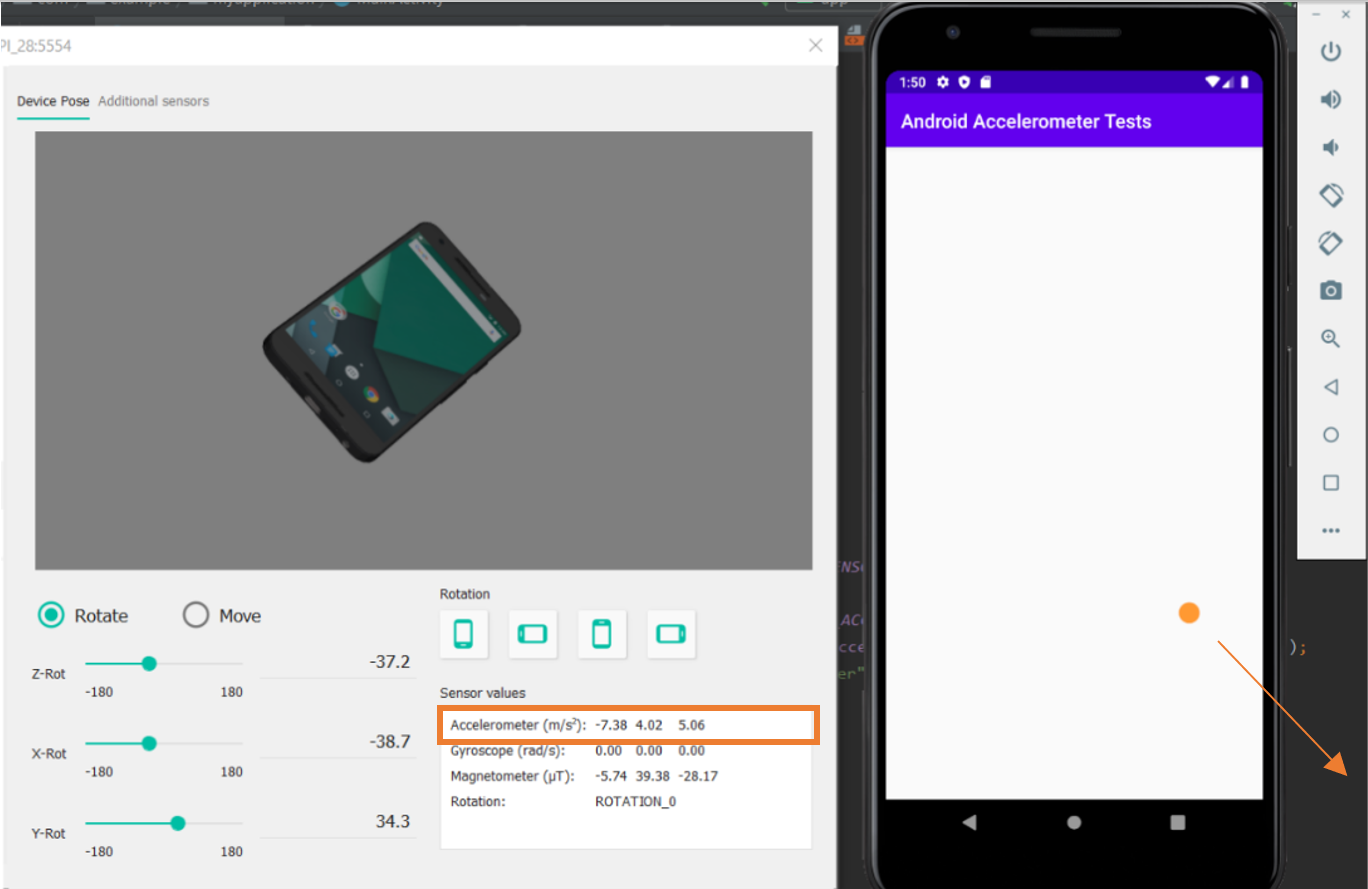
\includegraphics[width=0.9\textwidth]{img/ball-mov-test1.png}
\caption{\label{fig:ball-mov-test1}Accelerometer ball movement tests - case 1}
\end{figure}
%
\begin{figure}[!ht]
\centering
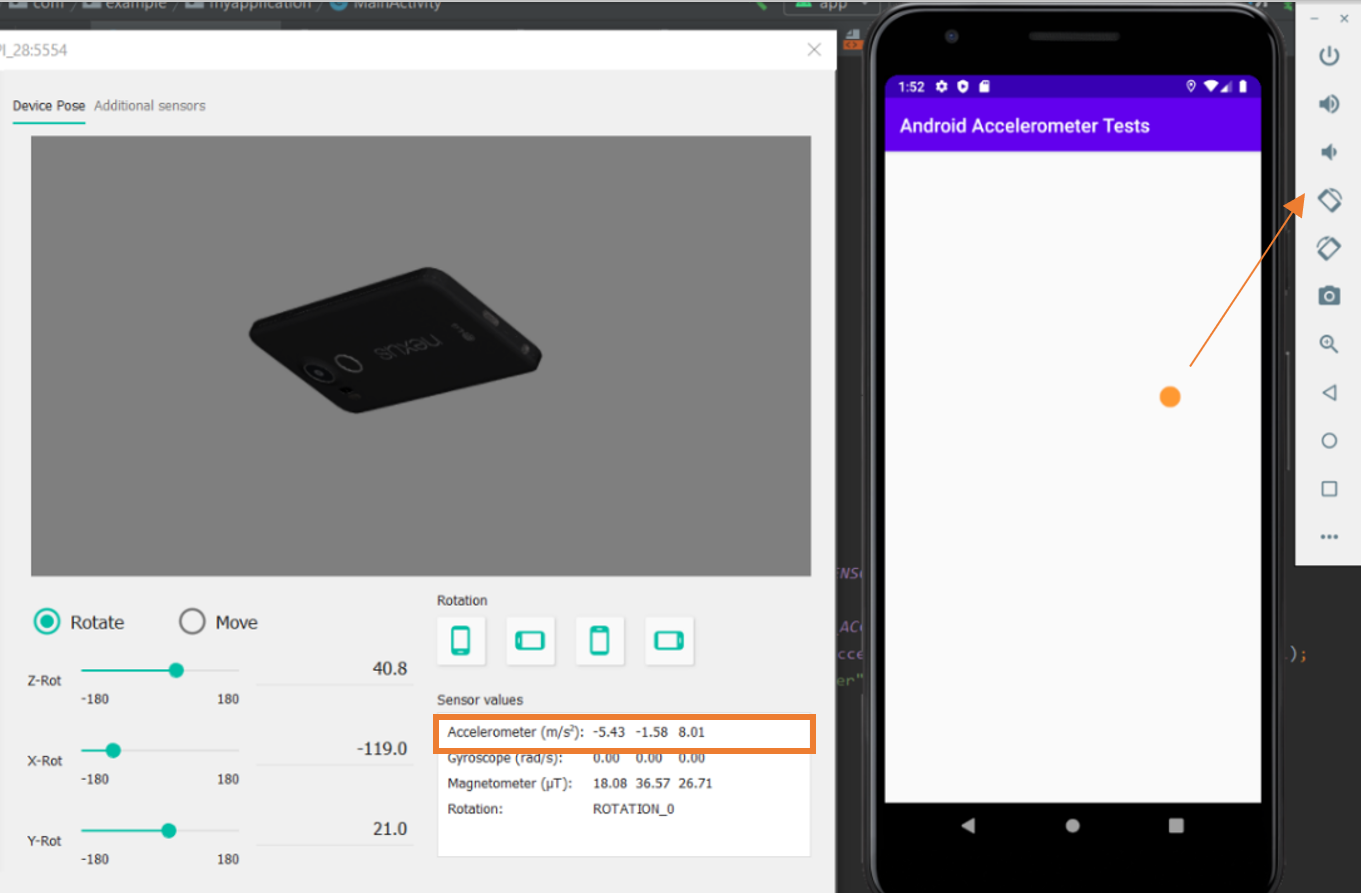
\includegraphics[width=0.9\textwidth]{img/ball-mov-test2.png}
\caption{\label{fig:ball-mov-test2}Accelerometer ball movement tests - case 2}
\end{figure}
%
As a way to test the code of the interaction with the rotation sensor, the values calculated were displayed on screen to perform a quick analysis, depicted in figure \ref{fig:rot-sens-test}. One must notice the method used based in control percentage values since it allows the use of different rover components maintaining the way these values are calculated.
%
\begin{figure}[!ht]
\centering
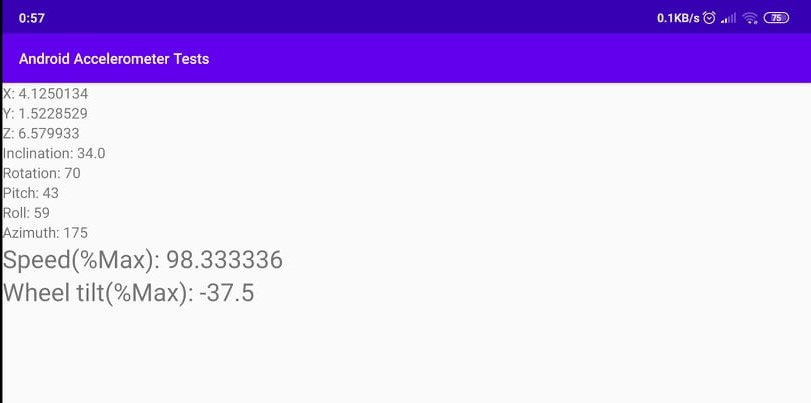
\includegraphics[width=0.7\textwidth]{img/rot-sensor-tests.png}
\caption{\label{fig:rot-sens-test}Rotation sensor tests}
\end{figure}
%